\documentclass[11pt]{article}

\usepackage[margin=1in]{geometry}
\usepackage{amsmath,amssymb,booktabs,array,graphicx}
\usepackage{tikz}
\usetikzlibrary{arrows.meta,positioning}
\usepackage[hidelinks]{hyperref}
\graphicspath{{docs/figures/}{figures/}}
\emergencystretch=3em
\setlength{\abovedisplayskip}{8pt}
\setlength{\belowdisplayskip}{8pt}

\title{A variational autoencoder,\\then two fraud notebooks}
\author{Notes on this repository}
\date{Recorded notebooks, seed 42}

\begin{document}
\maketitle

\begin{abstract}
This note is for someone new to the training loop.
Part~I derives a variational autoencoder without reference to fraud:
why a latent code is useful, why the marginal likelihood is an integral
you cannot compute, and how the ELBO, a diagonal Gaussian, and the
reparameterization trick make the model trainable.
Part~II specializes that model to anomaly detection and to the two
notebooks in this repo. Part~III says what each knob does, using the
runs we actually trained. Part~IV reports those runs and what they do
not show.

The synthetic notebook draws its own table. The Kaggle notebook uses the
public Credit Card Fraud Detection file. Neither number below is a
production false-positive budget.
\end{abstract}

\tableofcontents

\section{Part I --- VAE theory and mathematics}
\label{sec:part1}

\subsection{Symbols}

Every symbol below is used in the same way for the rest of the note.
$x$ is one observed row. $z$ is its latent code, a vector we do not observe.
$\theta$ is the decoder's weights. $\phi$ is the encoder's weights.

\begin{center}
\small
\begin{tabular}{@{}l>{\raggedright\arraybackslash}p{0.74\textwidth}@{}}
\toprule
Symbol & Meaning \\
\midrule
$p(z)$ & Prior. Here $\mathcal{N}(0,I)$, a standard Gaussian, fixed before training. \\
$p_{\theta}(x\mid z)$ & Decoder: how a code would generate a row. \\
$p_{\theta}(x)$ & Marginal likelihood of a row. An integral over every possible $z$. \\
$p_{\theta}(z\mid x)$ & True posterior. Proportional to $p_{\theta}(x\mid z)\,p(z)$. Intractable. \\
$q_{\phi}(z\mid x)$ & Encoder: a tractable stand-in for the posterior. \\
$\mu,\mathrm{logvar}$ & Mean and log-variance of the encoder Gaussian. \\
$\sigma$ & $\exp(\tfrac{1}{2}\mathrm{logvar})$, the standard deviation. \\
$\epsilon$ & Noise drawn from $\mathcal{N}(0,I)$, independent of $\phi$. \\
$\operatorname{ELBO}$ & Evidence lower bound. The training objective's ideal form. \\
$\beta$ & Weight on the KL term. The ideal ELBO uses $\beta=1$. \\
\bottomrule
\end{tabular}
\end{center}

\subsection{What an autoencoder is for}

A row of numbers is wide. Many of those numbers move together.
An autoencoder is a pair of functions that tries to keep what is shared
and throw away what is not. The encoder compresses $x$ into a shorter
code $z$. The decoder rebuilds a row $\hat{x}$ from $z$. Training
minimizes a reconstruction loss, some distance between $x$ and $\hat{x}$.
If the code is shorter than the row, the network cannot store every
detail, so it has to store the regularities that show up across many rows.

That is the whole idea, and it does not require a probability model.
The trouble shows up when you want to \emph{use} the code as a space,
not only as a bottleneck.

\subsection{Why a plain latent space is not a generative space}
\label{sec:islands}

Nothing in a plain autoencoder says where $z$ should live.
If a strange row is easier to rebuild from its own private code, the
encoder can park it on an island far from the codes of ordinary rows,
and the decoder can memorize that island. Reconstruction on the training
rows can still be excellent. Two things then fail.

First, a point halfway between two islands does not have to decode to
anything that looks like data. The line between two memorized codes can
pass through a region the decoder has never been asked to use.
Second, ``how typical is this code?'' has no answer. There is no prior,
so distance from the origin is not a measure of surprise. The latent
space is a lookup table with coordinates, not a smooth generative model.

A variational autoencoder adds a cost for that freedom. The encoder
must place $q_{\phi}(z\mid x)$ near a chosen prior, usually
$\mathcal{N}(0,I)$. Nearby codes are then forced to share one region,
and a point in that region is a place the decoder has been trained to
turn into a plausible row. Section~\ref{sec:picture} draws the two forces.
The KL term does not guarantee that a VAE will beat an autoencoder at
anomaly detection. It changes what the latent space means.

\subsection{A latent-variable model, and an integral you cannot do}

Write the row as something a hidden code could have produced.
The prior $p(z)=\mathcal{N}(0,I)$ says which codes are typical before
you see a row. The decoder $p_{\theta}(x\mid z)$ says which rows are
typical given a code. Together they define the marginal probability of
a row by summing over every code, weighted by how likely that code was:
\begin{equation}
\label{eq:marginal}
p_{\theta}(x)
= \int p_{\theta}(x\mid z)\, p(z)\, dz.
\end{equation}
The integral is the law of total probability. If you could compute it,
you could train $\theta$ by maximizing $\log p_{\theta}(x)$ on the rows
you have.

You cannot compute it here. $z$ is six-dimensional in both notebooks,
and the decoder is a stack of linear maps and ReLUs, not a density with
a closed integral. A grid over $\mathbb{R}^{6}$ is not a realistic
quadrature. Monte Carlo from the prior is the wrong sampler once
training has started: most prior samples are codes the decoder does not
associate with this particular $x$, so the average is dominated by
terms that are almost zero.

The posterior would be the right sampler. Bayes' rule says
\[
p_{\theta}(z\mid x)
= \frac{p_{\theta}(x\mid z)\,p(z)}{p_{\theta}(x)}.
\]
The denominator is the integral in \eqref{eq:marginal}. The distribution
you would need in order to train is defined using the quantity you are
trying to compute. That loop is why variational inference replaces the
posterior with a family you choose.

\subsection{Variational inference, and the ELBO two ways}
\label{sec:elbo}

Pick a family $q_{\phi}(z\mid x)$ that you can sample and whose density
you can evaluate. In this repo it is a diagonal Gaussian whose mean and
log-variance are the encoder outputs. It is not the true posterior.
It is a tractable approximation, and $\phi$ chooses which member of the
family is used for each $x$.

\paragraph{The identity.}
Start from the definition of the joint, $p_{\theta}(x,z)=p_{\theta}(x\mid z)\,p(z)$,
and from $\log p_{\theta}(x)=\log p_{\theta}(x,z)-\log p_{\theta}(z\mid x)$.
The left side does not depend on $z$, so an average over any $q_{\phi}(z\mid x)$
leaves it unchanged:
\begin{align}
\log p_{\theta}(x)
&= \mathbb{E}_{q_{\phi}}\!\left[\log p_{\theta}(x,z)-\log q_{\phi}(z\mid x)\right] \nonumber\\
&\quad + \mathbb{E}_{q_{\phi}}\!\left[\log q_{\phi}(z\mid x)-\log p_{\theta}(z\mid x)\right].
\label{eq:identity}
\end{align}
The second expectation is the KL divergence
$\mathrm{KL}\!\big(q_{\phi}(z\mid x)\,\|\,p_{\theta}(z\mid x)\big)$.
KL is zero when the two distributions are the same, and positive otherwise.
So the first expectation is a lower bound on $\log p_{\theta}(x)$, and the
gap is exactly how far the encoder is from the true posterior.

Expand the joint inside the first expectation:
\begin{equation}
\label{eq:elbo}
\begin{aligned}
\operatorname{ELBO}(x)
&= \mathbb{E}_{q_{\phi}}[\log p_{\theta}(x\mid z)]
 - \mathrm{KL}\!\big(q_{\phi}(z\mid x)\,\|\,p(z)\big).
\end{aligned}
\end{equation}
Equation \eqref{eq:identity} is then the sentence to remember:
\[
\log p_{\theta}(x)
= \operatorname{ELBO}(x)
+ \mathrm{KL}\!\big(q_{\phi}(z\mid x)\,\|\,p_{\theta}(z\mid x)\big).
\]
The reconstruction term, $\mathbb{E}[\log p_{\theta}(x\mid z)]$, says the
code you just drew has to explain the row. The KL against the prior says
the encoder cannot use an arbitrary island to do it. Maximizing the ELBO
pushes the gap $\mathrm{KL}(q\|p(\cdot\mid x))$ down at the same time,
because $\log p_{\theta}(x)$ does not depend on $\phi$ except through that
gap. When $q_{\phi}$ equals the true posterior, the gap is zero and the
ELBO equals $\log p_{\theta}(x)$.

\paragraph{Jensen's inequality.}
The same bound falls out of the integral directly. Insert $q_{\phi}$,
which integrates to one, into \eqref{eq:marginal}:
\[
\log p_{\theta}(x)
= \log \int q_{\phi}(z\mid x)\,
  \frac{p_{\theta}(x\mid z)\,p(z)}{q_{\phi}(z\mid x)}\, dz.
\]
The logarithm of an average is at least the average of the logarithm
(Jensen's inequality, because $\log$ is concave):
\begin{equation}
\label{eq:jensen}
\log p_{\theta}(x)
\ge
\mathbb{E}_{q_{\phi}}\!\left[
\log p_{\theta}(x\mid z)+\log p(z)-\log q_{\phi}(z\mid x)
\right].
\end{equation}
The right-hand side is \eqref{eq:elbo} again. Jensen tells you the ELBO
is a lower bound. The identity tells you what the missing piece is:
$\mathrm{KL}(q_{\phi}\|p_{\theta}(\cdot\mid x))$, which Jensen folds into
the inequality and does not name.

Training never touches $\log p_{\theta}(x)$ itself. It maximizes a
minibatch estimate of the ELBO, or a weighted surrogate of it, which is
what Part~II writes down for this code.

\subsection{A diagonal Gaussian, and the KL in closed form}
\label{sec:kl}

Let the encoder emit $\mu\in\mathbb{R}^{d}$ and
$\mathrm{logvar}\in\mathbb{R}^{d}$, and set
\[
q_{\phi}(z\mid x)
= \mathcal{N}\!\big(\mu,\ \operatorname{diag}(\exp(\mathrm{logvar}))\big).
\]
Coordinate $j$ has mean $\mu_{j}$ and variance $\sigma_{j}^{2}=\exp(\mathrm{logvar}_{j})$.
The prior $p(z)=\mathcal{N}(0,I)$ has the same independence and unit
variance. KL between diagonal Gaussians is the sum of the one-dimensional
KLs, so it is enough to derive one coordinate and then add.

Drop the index $j$. The log densities, up to the shared constant
$-\tfrac{1}{2}\log(2\pi)$, are
\begin{align*}
\log q(z)
&= -\tfrac{1}{2}\log \sigma^{2} - \frac{(z-\mu)^{2}}{2\sigma^{2}}, \\
\log p(z)
&= -\frac{z^{2}}{2}.
\end{align*}
The KL is $\mathbb{E}_{q}[\log q-\log p]$.
Under $q$, $(z-\mu)^{2}$ has expectation $\sigma^{2}$, so
\[
\mathbb{E}_{q}\!\left[\frac{(z-\mu)^{2}}{2\sigma^{2}}\right] = \tfrac{1}{2}.
\]
And $\mathbb{E}_{q}[z^{2}]=\mathrm{Var}_{q}(z)+\mu^{2}=\sigma^{2}+\mu^{2}$, so
\[
\mathbb{E}_{q}\!\left[\frac{z^{2}}{2}\right] = \tfrac{1}{2}\sigma^{2}+\tfrac{1}{2}\mu^{2}.
\]
Put those into the difference:
\begin{align*}
\mathrm{KL}(q\|p)
&= -\tfrac{1}{2}\log\sigma^{2} - \tfrac{1}{2}
   + \tfrac{1}{2}\sigma^{2} + \tfrac{1}{2}\mu^{2} \\
&= \tfrac{1}{2}\big(\mu^{2}+\sigma^{2}-1-\log\sigma^{2}\big).
\end{align*}
The $2\pi$ terms cancelled. Substitute $\sigma^{2}=\exp(\mathrm{logvar})$
and $\log\sigma^{2}=\mathrm{logvar}$, and multiply by $-1$ inside a
leading $-\tfrac{1}{2}$:
\begin{equation}
\label{eq:kl-1d}
\mathrm{KL}(q\|p)
= -\tfrac{1}{2}\Big(1+\mathrm{logvar}-\mu^{2}-\exp(\mathrm{logvar})\Big).
\end{equation}
Sum over the $d$ coordinates. That is the KL for one row.
\texttt{VAELoss} then averages over the batch, so a short batch and a
long batch report KL on the same scale:
\begin{equation}
\label{eq:kl-code}
\mathrm{KL}
= \frac{1}{B}\sum_{i=1}^{B}
\left(
-\tfrac{1}{2}\sum_{j=1}^{d}
\big(1+\mathrm{logvar}_{i,j}-\mu_{i,j}^{2}-\exp(\mathrm{logvar}_{i,j})\big)
\right).
\end{equation}
Two checks make the algebra trustworthy. If $\mu=0$ and $\mathrm{logvar}=0$,
then $\sigma^{2}=1$ and \eqref{eq:kl-1d} is zero: the encoder is the prior.
If $\mu=1$ and $\mathrm{logvar}=0$, \eqref{eq:kl-1d} equals $\tfrac{1}{2}$.
The code clamps $\mathrm{logvar}$ to $[-10,10]$ before this expression,
only so $\exp(\mathrm{logvar})$ cannot overflow. The clamp is not a model
of the data.

\subsection{The reparameterization trick}
\label{sec:reparam}

The reconstruction term is an expectation of a function of a sample $z$
drawn from $q_{\phi}$. A score needs a gradient with respect to $\mu$ and
$\mathrm{logvar}$. If the implementation draws $z$ from a Gaussian sampler
and then treats that draw as a constant, the sampler is a wall in the
autograd graph. The loss can change the decoder, but it cannot move the
distribution that produced the code. The sample's dependence on $\phi$
was thrown away at the draw.

Write the same Gaussian draw as a deterministic function of noise that
does not depend on $\phi$:
\begin{equation}
\label{eq:reparam}
\sigma=\exp\!\left(\tfrac{1}{2}\,\mathrm{logvar}\right),
\qquad
\epsilon\sim\mathcal{N}(0,I),
\qquad
z=\mu+\sigma\odot\epsilon.
\end{equation}
The symbol $\odot$ is elementwise multiplication.
$\partial z/\partial\mu=1$ and $\partial z/\partial\sigma=\epsilon$.
Gradients of the reconstruction with respect to $z$ flow straight into
the encoder. The KL term never needs $\epsilon$; \eqref{eq:kl-code} is
already a function of $\mu$ and $\mathrm{logvar}$.

A hand calculation, not a row from either notebook: one coordinate with
$\mu=1$, $\sigma=0.5$, and a draw $\epsilon=-1$. Then
$z=1+0.5\cdot(-1)=0.5$. If the reconstruction loss wants this coordinate
of $z$ to increase, it increases $\mu$ one-for-one. It also changes
$\sigma$ in the direction of $\epsilon$, which is negative on this draw,
so this particular sample asks the encoder to shrink $\sigma$ in order
to push $z$ up. A later draw with $\epsilon>0$ pushes $\sigma$ the other
way. Across a batch, $\sigma$ learns a width rather than chasing one
noise sample.

\texttt{TabularVAE.forward} is encode, then \eqref{eq:reparam}, then
decode. Scoring does not call \texttt{reparameterize}. It decodes $\mu$.
A fresh $\epsilon$ would change the score of a fixed row, and a threshold
fit on one set of draws would not refer to the next set.

\subsection{Which likelihood becomes which loss}

The ELBO's reconstruction term is an expected log-likelihood.
The loss you type is the negative of that term, plus the KL.

If the decoder is a Gaussian with fixed variance,
$\log p(x\mid z)=-\|x-\hat{x}\|^{2}/(2\sigma^{2})$ plus a constant that
does not depend on the prediction. Minimizing mean squared error is
exactly maximizing that likelihood. The variance only rescales the loss.
People often set it aside and minimize MSE directly.

If a coordinate of $x$ is a class index, the matching likelihood is
categorical. The decoder emits a logit for each class. The log-likelihood
of the observed class is the log of its softmax probability, and the
negative of that is the cross-entropy. \texttt{F.cross\_entropy} applies
the log-softmax to the raw logits. Putting a softmax in the module and
then another inside the loss would train a different, wrong objective.

Squared error on a class index is not a categorical likelihood. It invents
an order: class 9 would be nine times class 1. Merchant ids do not have
that order. Cross-entropy compares identity, not position on a line.

Part~II replaces the Gaussian MSE with Huber loss. The reason is
robustness, and the link back to a likelihood is written there. The KL
term does not care which reconstruction loss you used. It is still
\eqref{eq:kl-code}.

\subsection{The two forces on the code}
\label{sec:picture}

Reconstruction and the KL pull a code in opposite directions.
Reconstruction is happy to give an unusual row its own location if that
makes $\hat{x}$ closer to $x$. The KL charges for any $q_{\phi}$ that
leaves $\mathcal{N}(0,I)$: a mean far from the origin, or a variance far
from 1. Training stops at a compromise. Figure~\ref{fig:forces} is the
picture; $\beta$ in Part~III is the weight of the compromise.

\begin{figure}[ht]
\centering
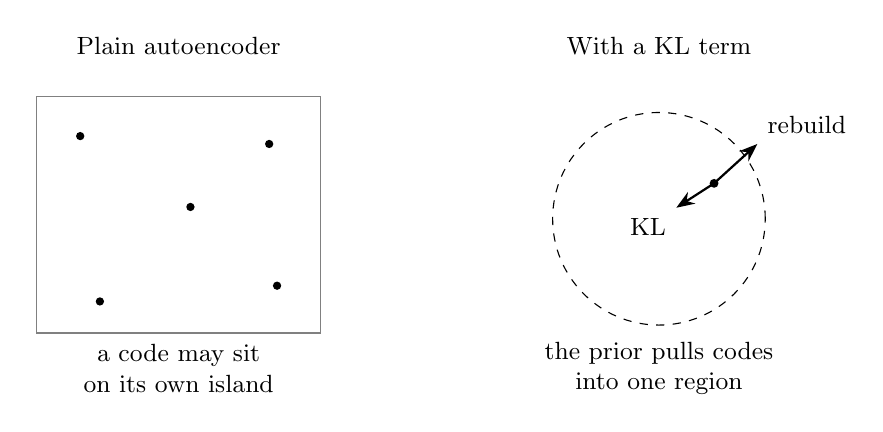
\begin{tikzpicture}[font=\small]
  \begin{scope}
    \node at (0,2.2) {Plain autoencoder};
    \draw[gray] (-1.8,-1.45) rectangle (1.8,1.55);
    \foreach \x/\y in {-1.25/1.05, 1.15/0.95, -1.0/-1.05, 1.25/-0.85, 0.15/0.15} {
      \fill (\x,\y) circle (1.5pt);
    }
    \node[align=center, text width=3.6cm] at (0,-1.9)
      {a code may sit on its own island};
  \end{scope}
  \begin{scope}[xshift=6.1cm]
    \node at (0,2.2) {With a KL term};
    \draw[dashed] (0,0) circle (1.35);
    \fill (0.7,0.45) circle (1.6pt);
    \draw[-{Stealth}, thick] (0.7,0.45) -- (1.25,0.95)
      node[above right] {rebuild};
    \draw[-{Stealth}, thick] (0.7,0.45) -- (0.22,0.14)
      node[below left] {KL};
    \node[align=center, text width=3.8cm] at (0,-1.9)
      {the prior pulls codes into one region};
  \end{scope}
\end{tikzpicture}
\caption{Left: reconstruction alone. Right: the same reconstruction arrow,
opposed by the KL. The dashed circle is a cartoon of $\mathcal{N}(0,I)$,
not a plot of either notebook.}
\label{fig:forces}
\end{figure}

\section{Part II --- Anomaly detection}
\label{sec:part2}

\subsection{Train on normal rows, score the rebuild}

The detector asks a narrower question than ``is this fraud?''
It asks whether a network that has only been asked to rebuild normal
rows finds this row hard. The fraud label is not an input to the loss.
After training, a normal row usually lands in the region the decoder
knows, and the residual is small. A row that breaks the normal patterns
is rebuilt as something more normal than it is, and the residual grows.

That fails in both directions. Fraud that looks ordinary in the columns
you kept reconstructs easily and stays under the cutoff. A legitimate row
that is merely new --- a distance or an amount the training window never
saw --- can score high. The score is conformity to the learned normal
structure. It is not a probability of fraud, and it is not evidence of
intent.

A second failure is contamination. If fraud is left in the training
normals, the decoder spends capacity on those patterns and the gap shrinks.
Both notebooks use labels to keep fraud out of the training window and
out of the calibration window. That is normal-only, or semi-supervised,
anomaly detection: labels build the reference set and score the holdout.
They do not appear in \texttt{VAELoss}. Calling the setup unsupervised
would be false.

\subsection{The synthetic notebook: mixed columns}
\label{sec:synthetic-design}

\texttt{generate\_synthetic\_transactions} draws 7{,}600 normal rows and
400 fraud rows (5\% of 8{,}000). Normal rows are tied together on purpose.
Fee tracks amount, rolling 24-hour spend falls as the gap since the last
transaction grows, device type follows distance from home, and merchant
id follows spend. Fraud is shifted off those links by a wide margin.
Recall of 1.0 on that table means the pipeline fired on a gap the
generator planted. It is not a claim about real card payments.

The continuous columns are \texttt{amount}, \texttt{fee},
\texttt{rolling\_spend\_24h}, \texttt{distance\_from\_home\_km}, and
\texttt{seconds\_since\_last\_txn}. All five are positive. The
preprocessor applies $\log(1+u)$ and then a z-score. Mean and population
standard deviation are fit on the 5{,}200 training normals only.
Merchant tokens \texttt{m0}--\texttt{m9} and device tokens
\texttt{chip}, \texttt{contactless}, \texttt{online} become one-hots
in that order. The encoder input is $5+10+3=18$ numbers.

The network is \texttt{TabularVAE} with latent size 6 and hidden width 64.
The encoder is $18\to 64\to 64$, then two linear maps to $\mu$ and
$\mathrm{logvar}$, each in $\mathbb{R}^{6}$. The decoder is
$6\to 64\to 64$, then three heads and no softmax: a linear head of width
5 for the scaled numbers, a logit head of width 10, and a logit head of
width 3. The split exists because the mistakes are different kinds.
Huber compares two real numbers. Cross-entropy compares a class identity.
One MSE head on a merchant index would invent the order the categorical
likelihood refuses.

Huber stands in for the Gaussian log-likelihood of Part~I, with a change
in the tails. With $\delta=1$,
\begin{equation}
\label{eq:huber}
\ell_{1}(r)=
\begin{cases}
\tfrac{1}{2} r^{2} & \text{if } |r|\le 1,\\
|r|-\tfrac{1}{2} & \text{if } |r|>1.
\end{cases}
\end{equation}
Inside one training standard deviation of the scaled column the penalty
is quadratic, the same shape as a Gaussian negative log-likelihood with
a fixed variance. Outside that band the penalty is linear, which is the
shape of a Laplace negative log-likelihood. The density whose negative
log is \eqref{eq:huber} is therefore Gaussian in the center and
exponential in the tails. The code does not fit a variance parameter.
$\delta=1$ is the choice that puts the kink at one standard deviation of
normal training traffic, after the log and the z-score. A raw amount
would let a few large but legitimate tickets dominate a pure square.

The quantity \texttt{VAELoss} differentiates is not the negative of
\eqref{eq:elbo} with a single density. It is the surrogate
\begin{equation}
\label{eq:train-loss}
\mathrm{total}
= \lambda_{\mathrm{cont}}\,\mathrm{Huber}
+ \lambda_{\mathrm{cat}}\,(\mathrm{CE}_{\mathrm{m}}+\mathrm{CE}_{\mathrm{d}})
+ \beta\,\mathrm{KL},
\end{equation}
with $\lambda_{\mathrm{cont}}=\lambda_{\mathrm{cat}}=1$ and $\beta=0.1$
in the synthetic notebook. The reductions, which are part of the
definition, are:

\begin{itemize}
\item Huber: \texttt{F.huber\_loss} with $\delta=1$ and
  \texttt{reduction="mean"}, so the mean runs over the batch and over the
  five continuous columns.
\item Each cross-entropy: mean over the batch. The two head-means are
  then added, so each categorical column contributes one batch-mean, not
  a mean that also divides by the number of classes.
\item KL: \eqref{eq:kl-code}, summed over the six latent coordinates and
  averaged over the batch.
\end{itemize}

A uniform guess on the two heads would score $\ln 10+\ln 3\approx 3.401$.
Epoch 1 printed cross-entropy 3.2698, just under that chance level.
Epoch 25 printed Huber 0.2116, cross-entropy 0.0861, and KL 5.8136.
The categories were being reconstructed by the end. The KL's role in the
weighted sum is Part~III.

The splits are disjoint by \texttt{row\_id}. Training is 5{,}200 normals
and is the only split that fits weights or the scaler. Calibration is
1{,}200 normals and is used once, for the threshold. Validation is the
remaining 1{,}200 normals plus all 400 fraud rows.

\subsection{How a row is scored}
\label{sec:score}

Training averages so that the step size does not grow with the batch.
A transaction needs one severity, so scoring sums the same pieces inside
the row. Decode $\mu$, not a sample. Drop the KL.
\begin{equation}
\label{eq:score}
\begin{aligned}
\mathrm{score}
&= \lambda_{\mathrm{cont}}\sum_{j}\ell_{1}(\hat{u}_{j}-\tilde{u}_{j})
 + \lambda_{\mathrm{cat}}\sum_{\mathrm{heads}}\mathrm{CE}(\mathrm{logits}, c).
\end{aligned}
\end{equation}
On the synthetic model the first sum has five terms and the second has
two. On the Kaggle model the second sum is empty: the categorical term
is a zero tensor, not a dummy class, and $\lambda_{\mathrm{cat}}$
multiplies zero. The lambdas and $\delta$ match training. The reduction
does not.

Arithmetic on the definition, not a real row: Huber terms 0.2 and 0.4
on a single row. The training reduction averages them to 0.3. The score
adds them to 0.6. Same residuals, same $\delta$, different question.

KL is a training regularizer. A large KL means the encoder is uncertain
or far from the prior, and that can be an anomaly score in another
system: threshold the KL itself, the prior density of $\mu$, or a density
fit on normal codes. Those answer ``how strange is the latent
distribution for this row.'' This repository answers ``how badly did the
normal-trained decoder rebuild this row.'' The calibration percentile is
a percentile of that rebuild error only.

Two hand-written checks in the synthetic notebook, not generator samples,
show the scale. An ordinary row scored about 0.052 and was not flagged.
A shifted row scored 25.95, of which about 15.90 was continuous Huber,
3.79 was the merchant cross-entropy, and 6.26 was the device
cross-entropy. The device term is large because a far-from-home chip
purchase disagrees with a decoder trained on local chip use.

\subsection{The percentile is a false-positive budget}
\label{sec:threshold}

\texttt{fit\_threshold} scores a pure-normal calibration window and stores
one order statistic. A 95th percentile is a budget of about 5\% of normal
traffic. A 99th percentile is a budget of about 1\%. The comparison at
decision time is $\mathrm{score}\ge\mathrm{threshold}$. Later calls read
the stored float. They do not recompute a percentile on the request, and
they do not look at holdout fraud.

``About'' is deliberate. On the calibration sample the flag rate is near
$(100-p)/100$, not identical to it, because a finite-sample percentile
and a $\ge$ rule do not flag exactly $1-p/100$ of those same rows.
On a \emph{different} normal sample the rate moves again. In the synthetic
notebook the validation normals' own 95th percentile was 2.040, under the
calibration cutoff 2.1162, and 4.4\% of them were flagged rather than 5\%.
The Kaggle holdout is also later in time, so its normals are not a second
draw from the calibration window. Section~\ref{sec:kaggle-results} records
the rate that actually occurred.

The scorer refuses to fit a threshold on a frame that contains fraud, and
it refuses a calibration set smaller than 200 rows. Both guards are there
so a percentile is not fit on the wrong population or on a handful of
order statistics.

\subsection{The Kaggle notebook: thirty continuous columns}
\label{sec:kaggle-design}

The public file \texttt{creditcard.csv} has 284{,}807 rows and 492 fraud
labels (0.1727\%). Columns are \texttt{Time}, \texttt{V1}--\texttt{V28},
\texttt{Amount}, and \texttt{Class}. \texttt{V1}--\texttt{V28} are
principal components the dataset authors computed and released without
the loading matrix. A large \texttt{V14} is not a merchant or a country.
Standardizing those columns again is for the Huber scale. It is not a
second scientific PCA.

The split sorts by \texttt{Time}, breaking ties by row order, then cuts
by position: the first 60\% of rows is the training window, the next 20\%
is calibration, and the last 20\% is the mixed holdout. Fraud inside the
first two windows is dropped, not moved into the holdout. The recorded
cut left 170{,}524 training normals (360 fraud rows excluded), 56{,}904
calibration normals (57 fraud rows excluded), and a holdout of 56{,}887
normals plus 75 frauds. Most fraud in this file sits early, so the
holdout has far fewer than 20\% of the 492 labels. \texttt{MAX\_TRAIN\_NORMALS}
was \texttt{None}: every training-window normal was used.

Preprocessing, fit on those training normals only:

\begin{itemize}
\item \texttt{Amount} is $\log(1+u)$, then z-scored. Zero is a real amount,
  and $\log(1+0)=0$.
\item \texttt{Time} is z-scored and not logged. It is seconds from the
  first row, a clock that starts at 0.
\item \texttt{V1}--\texttt{V28} are z-scored with the training-normal mean
  and population standard deviation. They are signed, so $\log(1+u)$ does
  not apply.
\end{itemize}

The model is the same class with \texttt{cat\_cardinalities} empty:
30 inputs, latent size 6, hidden width 128, no categorical head.
$\beta=0.01$, $\delta=1$, twelve epochs, Adam with learning rate $10^{-3}$,
batch size 1{,}024. The training loss is \eqref{eq:train-loss} with the
cross-entropy term equal to zero. The score is the sum of the thirty
Huber terms. The operating threshold is the 99th percentile of
calibration scores, not the 95th. A 5\% normal flag rate would be
thousands of alarms on a fraud rate well under 1\%.
Section~\ref{sec:percentile} prints the neighbors of that choice.

\section{Part III --- What the knobs do}
\label{sec:part3}

\subsection{Beta, and what happened when we changed it}
\label{sec:beta}

In \eqref{eq:elbo} the KL has weight 1. A $\beta$-VAE keeps the same
terms and multiplies the KL by $\beta$. Nothing else about the
derivation changes. $\beta$ is the price of a code that leaves the prior.

If $\beta\to 0$, the price disappears. The model approaches a plain
autoencoder that still happens to emit $\mu$ and $\mathrm{logvar}$.
Reconstruction can improve, and the latent space can go back to the
islands of Section~\ref{sec:islands}. Interpolation stops being meaningful
because nothing paid for a shared region. Anomaly detection can still
work when the bottleneck alone is enough, which is why a small $\beta$
is not automatically a bug. It does give up the reason Part~I gave for
using a VAE.

If $\beta$ is large, the prior wins. The encoder sets
$q_{\phi}(z\mid x)\approx\mathcal{N}(0,I)$ for every row, so $z$ carries
almost no information about $x$. The decoder, seeing only that
uninformative code, outputs something close to the mean of the training
rows. Every row is rebuilt in nearly the same way. Reconstruction error
then measures distance from the mean, and if the decoder has collapsed
all the way, even that signal flattens: the score stops separating
unusual rows from ordinary ones. This is posterior collapse. The name
refers to $q_{\phi}$, which has collapsed onto the prior, not to the
anomaly score directly. The score goes quiet because the code went quiet.

The synthetic run used $\beta=0.1$, width 64, latent size 6, 25 epochs.
Epoch 25 printed Huber 0.2116, cross-entropy 0.0861, and KL 5.8136.
The weighted pieces are 0.2116, 0.0861, and $0.1\times 5.8136=0.5814$.
The regularizer was larger than Huber plus cross-entropy (0.2977) in the
training loss. It had not erased them. The categories were far below the
chance level 3.401 from Part~II, and Part~IV shows that the planted fraud
was still easy to flag. $\beta=0.1$ was a real compromise on that table,
not a collapse.

The Kaggle table is a harder compromise. After per-column standardization,
\texttt{V1}--\texttt{V28} are only weakly dependent, and a 6-dimensional
code cannot rebuild 30 such columns faithfully. With $\beta=0.1$ and
width 64 the prior won immediately. A diagnostic fit on the same
training window, seed 42, batch 1{,}024, and Adam at $10^{-3}$, reached
Huber 0.3456 and KL 0.0001 by epoch 4. The Huber of predicting the
scaled training mean, a vector of zeros, is 0.3469 on that window.
The encoder's means on a training batch had standard deviation about
0.003. The code was unused, and the loss was the mean predictor.

The notebook therefore uses $\beta=0.01$ and width 128. Epoch 12 printed
Huber 0.1382 and KL 7.9357, so the weighted KL is
$0.01\times 7.9357=0.0794$, smaller than the Huber term. Huber 0.1382
is also well under the mean-predictor value 0.3469, which is the check
that $z$ is doing some work. It is not a claim that twelve epochs found
the best $\beta$. The curve was still falling by about 0.002 per epoch
at the end (0.1440 at epoch 9, 0.1382 at epoch 12). Twelve epochs is the
budget of the recorded run.

Two standard remedies are not in this repo. KL annealing starts $\beta$
near 0 so the decoder learns a reconstruction, then raises $\beta$.
Free bits allow each latent coordinate a small KL budget before the
penalty turns on, so the encoder can keep a little information. Either
would change the training loop. The notebooks use a constant $\beta$.

\subsection{The other knobs}
\label{sec:percentile}

\paragraph{Latent dimension.}
This is the width of $z$, 6 in both notebooks. Too small, and normal
patterns that the decoder could have used are thrown away, so ordinary
rows look anomalous. Too large, and the code can memorize, which is the
island problem with a wider table. Six is a bottleneck on the 18-wide
synthetic input. On the 30 Kaggle columns it is a severe one, which is
why beating the mean predictor mattered more than the raw Huber value.

\paragraph{Hidden width.}
This is the width of the trunk, 64 in the synthetic notebook and 128 in
the Kaggle notebook. Too narrow, and the maps from $x$ to $(\mu,\mathrm{logvar})$
and back cannot fit the normal patterns; the loss sits near a constant.
Too wide, and you buy capacity the latent bottleneck may not use.
The synthetic notebook uses width 64 at $\beta=0.1$ and separated the
planted gap. The same width at $\beta=0.1$ collapsed on the Kaggle
table; the run that learned used width 128 together with $\beta=0.01$.
Those two changes were not crossed as a full grid. The evidence is the
pair of fits in Section~\ref{sec:beta}, not a claim that width alone
was the cause.

\paragraph{Huber delta.}
$\delta$ is the width of the quadratic region in \eqref{eq:huber}, in
units of the scaled columns. Both notebooks use $\delta=1$. Smaller, and
almost every residual is in the linear regime, so small errors barely
move the gradient. Larger, and the loss looks more like MSE, so a few
huge residuals dominate. Because the columns are z-scored, $\delta=1$
means ``one training standard deviation,'' which is the scale the rest
of the pipeline assumes. Changing $\delta$ at score time without changing
it in training would make the threshold refer to a different loss.

\paragraph{Lambda weights.}
$\lambda_{\mathrm{cont}}$ and $\lambda_{\mathrm{cat}}$ scale Huber and
cross-entropy in both \eqref{eq:train-loss} and \eqref{eq:score}.
Both are 1. On the mixed model, lowering $\lambda_{\mathrm{cat}}$ tells
the decoder it may ignore merchant and device. Raising it lets a wrong
merchant swamp a wrong amount. On the Kaggle model $\lambda_{\mathrm{cat}}$
multiplies zero. It is left at 1 so the same \texttt{LossConfig} fields
exist; it does not change the Kaggle score.

\paragraph{Threshold percentile.}
Section~\ref{sec:threshold} is the definition. The synthetic notebook
stores the 95th percentile, printed 2.1162. The Kaggle notebook stores
the 99th, printed 34.7925. The table below is the Kaggle reconstruction
score at four calibration percentiles. Holdout fraud was not used to
pick the row. The 99th percentile is the operating point because the
95th flags about 5\% of normals (here, normal FPR 0.0497) for a holdout
that contains 75 frauds among 56{,}962 rows.

\begin{center}
\small
\begin{tabular}{@{}rrrrrr@{}}
\toprule
Pct & Threshold & Precision & Recall & F1 & Normal FPR \\
\midrule
95   & 14.2839 & 0.0208 & 0.8000 & 0.0405 & 0.0497 \\
97   & 18.2676 & 0.0398 & 0.8000 & 0.0758 & 0.0255 \\
99   & 34.7925 & 0.0998 & 0.5333 & 0.1681 & 0.0063 \\
99.5 & 50.4868 & 0.1461 & 0.3467 & 0.2055 & 0.0027 \\
\bottomrule
\end{tabular}
\end{center}

Moving from 95 to 99 cuts recall from 0.80 to 0.53 and lifts precision
from 0.02 to 0.10. That is the trade the percentile \emph{is}.
The normal FPR at the 99th percentile is 0.0063, under the 1\% budget,
because the holdout normals are a later slice of time rather than a
reshuffle of the calibration window.

\paragraph{Epochs and learning rate.}
Both notebooks use Adam with learning rate $10^{-3}$. Too high, and the
loss diverges. The code clamps log-variance to $[-10,10]$ so one bad step
cannot overflow the KL. The recorded losses stayed finite, which is all
that printout shows; it is not a sweep of the learning rate.
Too low, and Huber is still near its starting value when the epoch budget
ends. The synthetic notebook runs 25 epochs at batch size 128.
The Kaggle notebook runs 12 epochs at batch size 1{,}024.
Batch size changes the noise of the gradient, not the definition of
\eqref{eq:score}. The Kaggle Huber was still declining at epoch 12, so
that budget is not a claim of convergence.

\begin{center}
\footnotesize
\begin{tabular}{@{}l>{\raggedright\arraybackslash}p{0.24\textwidth}>{\raggedright\arraybackslash}p{0.22\textwidth}>{\raggedright\arraybackslash}p{0.28\textwidth}@{}}
\toprule
Knob & Too low & Too high & Recorded choice \\
\midrule
$\beta$ &
islands, prior unused &
collapse onto $\mathcal{N}(0,I)$ &
0.1 synthetic; 0.01 Kaggle \\
latent size &
normal rows look odd &
room to memorize &
6 in both \\
hidden width &
underfit trunk &
capacity the code may ignore &
64 synthetic; 128 Kaggle \\
$\delta$ &
almost all linear &
tails act like MSE &
1, in scaled units \\
$\lambda_{\mathrm{cont}},\lambda_{\mathrm{cat}}$ &
that head is ignored &
that head swamps the other &
both 1 \\
percentile &
many normal flags &
misses moderate fraud &
95 synthetic; 99 Kaggle \\
epochs, Adam lr &
Huber barely moves &
unstable, or no further gain &
25 / 12 epochs, lr $10^{-3}$ \\
\bottomrule
\end{tabular}
\end{center}

\section{Part IV --- Results, without the gloss}
\label{sec:part4}

\subsection{The synthetic run is a sanity check}

Validation, and only validation, produced the classification report.
Positive class is fraud. The threshold was the calibration 95th
percentile, 2.1162.

\begin{center}
\small
\begin{tabular}{@{}lrrrr@{}}
\toprule
Class & Precision & Recall & F1 & Support \\
\midrule
Normal & 1.000 & 0.956 & 0.977 & 1200 \\
Fraud  & 0.883 & 1.000 & 0.938 & 400 \\
\bottomrule
\end{tabular}
\end{center}

Accuracy was 0.967. Every synthetic fraud row scored above the cutoff
(the lowest fraud score in validation was 13.189; the cutoff was 2.1162).
Fraud precision is 0.883 rather than 1 because 4.4\% of the validation
normals were also flagged. With 400 true positives, that precision is
400 true positives and 53 false positives, and $53/1200=0.044$.

The score distributions explain why this was easy. Validation normals had
median 0.667 and a 95th percentile of 2.040. Validation fraud had median
24.344 and a minimum of 13.189. The generator put fraud several standard
deviations off the normal links, in the scaled inputs as well as in the
score. A pipeline that could not separate that gap would be broken.
Separating it does not mean the same weights would separate a subtle
fraud, and it does not mean the table was a real card extract.

\subsection{The Kaggle holdout}
\label{sec:kaggle-results}

The operating comparison is the 99th percentile of each model's
calibration scores. The VAE score is summed Huber. The Isolation Forest
is fit on the same scaled training normals, with 100 trees and sklearn's
default \texttt{max\_samples} (256 rows per tree). Its anomaly score is
the negation of \texttt{decision\_function}, so larger means more
anomalous. Its threshold is not the forest's \texttt{contamination}
default and was not fit on holdout fraud.

\begin{center}
\small
\begin{tabular}{@{}lrrrrrr@{}}
\toprule
Model & Precision & Recall & F1 & PR-AUC & ROC-AUC & Normal FPR \\
\midrule
VAE & 0.0998 & 0.5333 & 0.1681 & 0.0809 & 0.9384 & 0.0063 \\
Isolation Forest & 0.0470 & 0.2267 & 0.0778 & 0.0382 & 0.9528 & 0.0061 \\
\bottomrule
\end{tabular}
\end{center}

At that shared false-positive budget the VAE is the better detector on
this split: higher precision, recall, F1, and PR-AUC. The forest's
ROC-AUC is slightly higher (0.9528 against 0.9384). Those two facts can
be true together, and the next paragraphs say why.

VAE confusion at threshold 34.7925: TN 56{,}526, FP 361, FN 35, TP 40.
Forest confusion at its own 99th percentile: TN 56{,}542, FP 345, FN 58,
TP 17. The holdout base rate is $75/56962\approx 0.0013$.

Accuracy is the wrong summary. The VAE's accuracy is 0.993.
Calling every row normal is $56887/56962\approx 0.9987$, which is higher,
because the VAE spends 361 false positives to buy 40 true positives.
A silent detector wins on accuracy whenever fraud is this rare.
The number is printed in the notebook so that this comparison is easy to
make, not so that 0.993 can be quoted as performance.

ROC-AUC and PR-AUC answer different questions.
ROC-AUC is the probability that a random fraud scores above a random
normal. It can look strong, here 0.94, when the typical fraud outranks
the typical normal, even if most rows above a useful cutoff are still
normal. PR-AUC is average precision across thresholds. A ranker that
ignores the features and scores at random has PR-AUC equal to the base
rate, about 0.0013. The VAE's 0.0809 is well above that, so the ranking
is real, and it is still a low precision: at the operating point only
about one flagged row in ten is fraud. The forest's higher ROC-AUC with
a lower PR-AUC is the same phenomenon in the comparison. ROC rewards
ordering in the bulk of the normals. Precision-recall cares what happens
in the tail you would actually flag.

Figure~\ref{fig:scores} is that tail. The dashed line is the frozen
calibration cutoff. The full-range panel is dominated by the normal mass
near small scores and by a long fraud tail. The zoom is there so the
cutoff is visible.

\begin{figure}[ht]
\centering
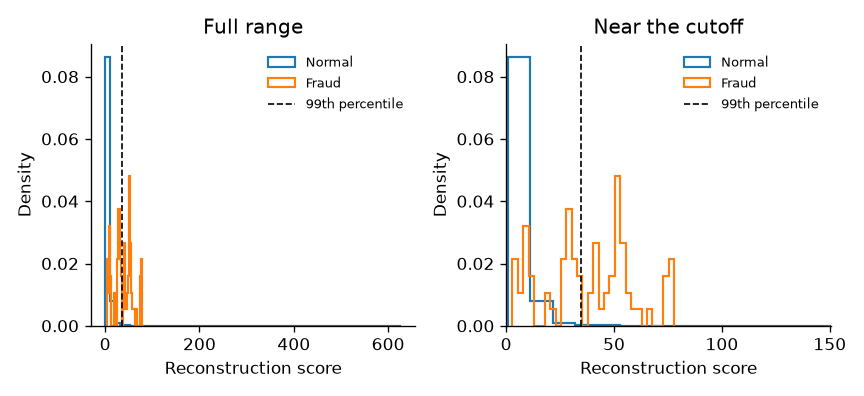
\includegraphics[width=\textwidth]{kaggle_score_hist.png}
\caption{Holdout reconstruction scores from the Kaggle notebook's
training procedure (seed 42, $\beta=0.01$, width 128, 12 epochs).
The dashed line is the 99th percentile of calibration normals, 34.7925.}
\label{fig:scores}
\end{figure}

\subsection{What the latent picture can show}

Figure~\ref{fig:latent} is not \texttt{V1} against \texttt{V2}.
The axes are a second PCA, fit on 8{,}000 normal-training latent means
and then applied to the holdout. In the recorded run those two axes
explained 0.227 and 0.179 of the variance of the \emph{codes}, not of
the original columns. The scatter shows 4{,}000 holdout normals and all
75 holdout frauds. Normals were downsampled for readability. Fraud was
not.

\begin{figure}[ht]
\centering
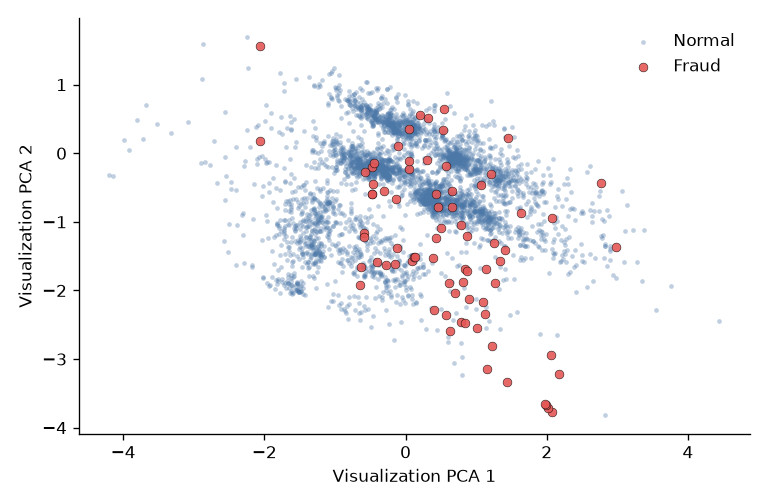
\includegraphics[width=0.92\textwidth]{kaggle_latent_class.png}
\caption{Evaluation codes $\mu\in\mathbb{R}^{6}$, projected for display.
The projection was not fit on fraud or on the holdout. Many fraud points
sit inside the normal cloud. The training target was reconstruction under
a KL penalty, not separation on this plane.}
\label{fig:latent}
\end{figure}

A visible gap would be encouraging and still would not be the objective.
The absence of a clean gap is also informative: a 2D cartoon of a 6D
code will hide directions that the reconstruction score uses.
Do not read a cluster in this plot as a fraud mode the model discovered.
The class colors are the hidden labels, drawn after scoring.

\subsection{Limits, and what would be next}

The synthetic fraud shift is large on purpose. The Kaggle file is a real
public extract, and it is still one European card program from 2013,
with features that have already been replaced by someone else's PCA.
A model that ranks this holdout has not been shown to rank a later year,
another issuer, or a table whose columns still have names.

\begin{itemize}
\item The category sets in the synthetic model are closed. An unseen
  merchant id is rejected. It is not given a score and it is not labeled
  fraud. The Kaggle model has no categories at all.
\item Each row is independent. There is no cardholder, no account, and
  no sequence. \texttt{Time} is seconds from the first row.
  \texttt{seconds\_since\_last\_txn} and \texttt{rolling\_spend\_24h}
  in the synthetic table are columns, not a hidden state.
\item Labels were used to build the normal windows. That is a cleaner
  reference than a raw extract, and it means a wrong label, or fraud left
  in the ``normal'' rows, teaches the decoder to rebuild the thing you
  hoped it would miss.
\item The cutoff drifts when normal behavior drifts. 2.1162 and 34.7925
  belong to the calibration windows that produced them. A later window
  needs its own percentile, fit on normals that were not used to train,
  and then frozen again.
\item The score is not a probability. Crossing the cutoff means ``at or
  above the stored percentile.''
\item $\beta$ is constant. Annealing and free bits were not tried.
  The Kaggle Huber curve had not flattened at epoch 12.
\item The latent picture is a visualization PCA. It is not the dataset's
  \texttt{V1}--\texttt{V28}, and it was not the training target.
\end{itemize}

The mixed-data design is the one that would meet a table such as
IEEE-CIS, where a transaction carries both amounts and high-cardinality
ids. The synthetic notebook is a small version of that shape, not that
dataset. Embeddings would replace the one-hot merchant head once the
vocabulary no longer fits in ten columns. KL annealing is the first
training change if a new table collapses the way $\beta=0.1$ did here.
Drift monitoring is a scheduled refit of the percentile on fresh normals,
not a new model class. Serving is the frozen preprocessor, the state
dict, and the stored threshold: \texttt{ReconstructionScorer.score}
already implements that contract for one row, and it does not retrain.

\end{document}
